\chapter{Method (draft)}
\label{chap:method}
In this chapter, we discuss the proposed methodology by describing the employed recommender framework and the different algorithms that are plugged into it.

\section{Framework (TODO - insert references)}
Due to the infeasibility of deploying a live recommender on NU.nl, we opt for offline evaluation that simulates the online environment. In an online scenario, the query for a recommendation is generated every time the user logs in or whenever a user views a news article. But, this implicit data is absent and what we posses are the comments as interactions.

Therefore, one crucial assumption we make is that the moment the user comments is the moment he queried for a recommendation. So we consider the brief time period before a comment is when a query for recommendations was made. We had also previously reported in Chapter~\ref{chap:data} that the average span between the time of article publication and the last comment was close to 32 hours (TODO-cross check). This in a simple way, is an indicator of how far back we must look and what would be considered as fresh. We go into much more detail regarding freshness in this scenario in Section~ (TODO- insert section). These fresh items are then treated as the candidate items for our recommender.

To summarize, for each comment we would retrieve the recent articles before the comment's time point then rank them through our recommender and verify if the target item is in the top of our ranked list of items. The model of the recommender itself is trained over the interactions preceding the comment's time point. We investigate how far back to look for training the model in Section~ (TODO- insert section). Figure~\ref{fig:frame} illustrates the recommender framework.

\begin{figure}[!h]
\centering
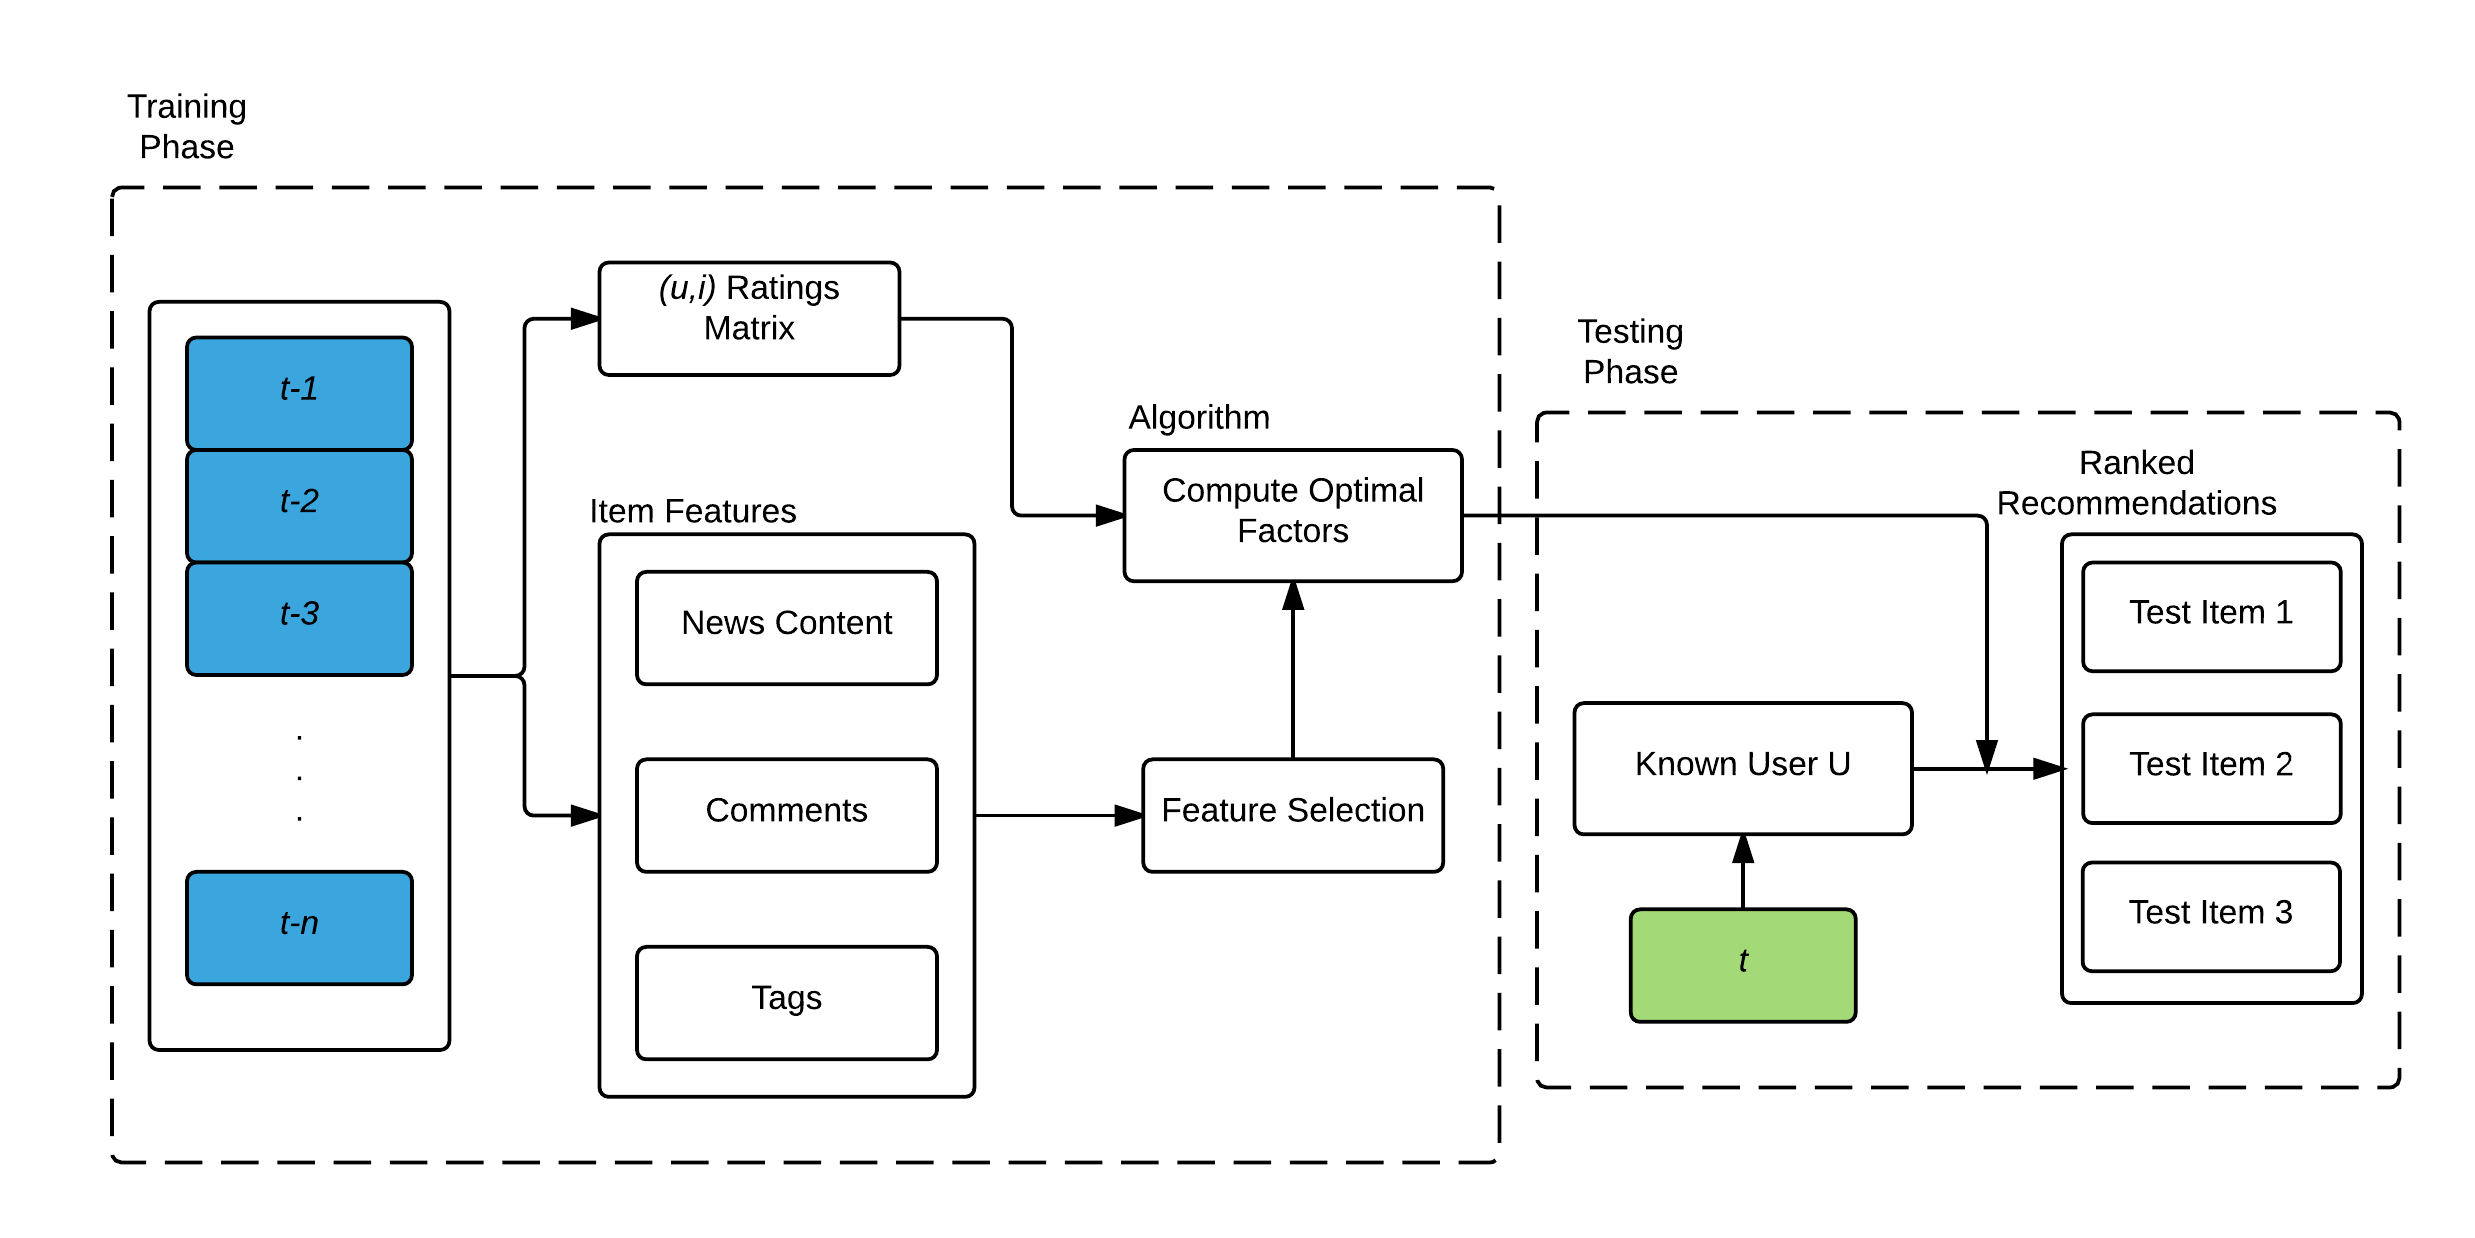
\includegraphics[width=0.85\textwidth]{c-method_images/frame.png}
\caption{Framework}
\label{fig:frame}
\end{figure}

\section{Feature Engineering}

\section{Algorithm}
\cite{rendle_factorization_2012}
\subsection{SVD++}
\cite{koren_factorization_2008}
\subsection{gSVD++}
\cite{manzato_gsvd++:_2013}

